\documentclass[a4paper,12pt]{article}

\usepackage[utf8]{inputenc}
\usepackage[ngerman]{babel}
\usepackage[T1]{fontenc}
\usepackage{graphicx}
\usepackage[cache=false]{minted}
\usepackage{dirtree}

\begin{document}
\begin{titlepage}
    \begin{center}
        \vspace*{1cm}
        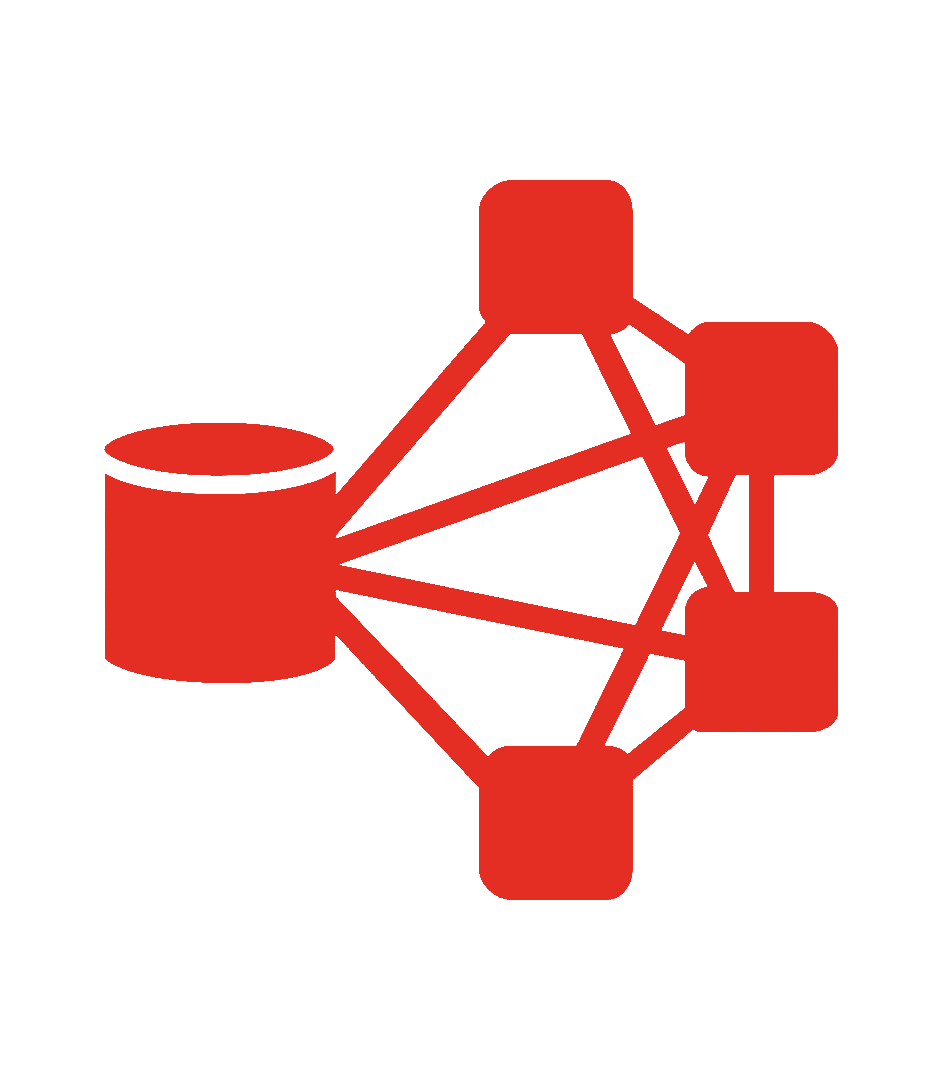
\includegraphics[width=10cm]{Logo.png}
        
        \textbf{\huge MapReduce-System}
        
        \vspace{0.5cm}
        NVS Projekt 2
                 
        \vspace{1.0cm}
    
        \textbf{Alexander Grill 5CHIF}
        
        \today
        
        \vfill
                 
                 
        \vspace{0.5cm}
                 
        Informatik\\
        HTBLUvA Wr.Neustadt\\
        Österreich\\

                 
    \end{center}
\end{titlepage}  
\newpage
\tableofcontents
\newpage


\section{Einführung}

\subsection{Vorwort}

\subsection{Motivation}

\section{Aufgabenstelllung}

\subsection{Erläuterung der Grundproblematik}

\subsection{Idee}

\subsection{Themenbereiche}

\section{Grundlagen}

\subsection{Was ist ein MapReduce System?}
Das Verfahren wurde 2004 von Google entwickelt für die Indexierung von Webseiten. Das Framework wird bei Datenbanken eingesetzt und dient zur Verarbeitung von großen, komplexen, unstrukturierte Datenmengen.
Dieses Verfahren findet Anwendung für BigData und Datawarehouse, weil in solchen Fällen große Datenmengen in kürzester Zeit mittels Software verarbeitet, analysiert, aggregiert als auch kompremiert werden. 
Map Reduce parallelisiert die Bearbeitung, durch die Verteilung auf mehrere gleichzeitig auszuführende Tasks. Der Grund, warum dieses Framework solche Datenmengen verarbeiten kann ist, weil die Aufgaben auf mehreren Rechnern aufgeteilt werden. Jeder einzelne Rechner startet Prozesse, die Parallel die Daten verarbeitet und auswertet.
Ein einzelner Rechner stoßt schnell an seine Grenzen, deshalb ist die Verarbeitung von Daten, mittels mehreren Knoten sehr effizient und bietet eine bessere Performance.

\subsection{Map und Reduce}
Die beiden Grundfunktionen Map und Reduce, für das Verfahren, sorgen für die Aufteilung der Aufgaben in kleinere parallelisierten Arbeitspakete und führen am Ende die Ergebnisse zusammen. Bei großen relationalen Datenbanken und komplexen Queries lassen sich typische Problem, bezglüch Verarbeitung von großen Datenmengen beseitigen.
Die Map Funktion, verteilt die Aufgaben an unterschiedlichen Knoten eines Clusters. Die Reduce Funktion sortier die verfassten Ergebnisse und fügt sie am Ende wieder zusammen.
Zwischen den zwei Funktionen gibt es auch die Shuffel Phase, in dieser werden den Zwischenergebnisse mit einem Schlüssel versehen, sodass diese auf dem jeweiligen Computersystem verarbeitet werden.
\section{Umsetzung}

\subsection{Aufbau}

\subsection{Klassendesign}

\subsection{Source Code Dokumentation}

\subsection{Verwendete Bibliotheken}

\section{Anwendungsfälle}

\section{Schlusswort}

\section{Referenzen}

\end{document}
